\documentclass[12pt]{article}
\usepackage{fullpage}

\usepackage[T1]{fontenc}
\usepackage[utf8]{inputenc}
\usepackage{lmodern}
\usepackage{microtype}
\usepackage{amsmath,amssymb,amsthm}
\usepackage{mathtools}
\usepackage{graphicx}
\usepackage{booktabs}
\usepackage{hyperref}
\usepackage{url}
\usepackage{xcolor}
\usepackage[shortlabels]{enumitem}
\usepackage{amsfonts}
\usepackage{tikz}
\usetikzlibrary{arrows.meta,positioning,shapes.geometric,calc}

\hypersetup{colorlinks=true,linkcolor=blue,citecolor=blue,urlcolor=blue}

\theoremstyle{plain}
\newtheorem{theorem}{Theorem}
\newtheorem{proposition}[theorem]{Proposition}
\newtheorem{lemma}[theorem]{Lemma}
\newtheorem{corollary}[theorem]{Corollary}

\theoremstyle{definition}
\newtheorem{definition}[theorem]{Definition}

\theoremstyle{remark}
\newtheorem*{remark}{Remark}

\newcommand{\R}{\mathbb{R}}
\newcommand{\bH}{\mathbf{H}}
\newcommand{\bP}{\mathbf{P}}
\newcommand{\bb}{\mathbf{b}}
\newcommand{\bv}{\mathbf{v}}
\newcommand{\bw}{\mathbf{w}}
\newcommand{\bp}{\mathbf{p}}
\newcommand{\bq}{\mathbf{q}}
\newcommand{\br}{\mathbf{r}}
\newcommand{\by}{\mathbf{y}}
\newcommand{\bu}{\mathbf{u}}
\newcommand{\bk}{\mathbf{k}}
\newcommand{\bz}{\mathbf{z}}
\newcommand{\bs}{\mathbf{s}}
\newcommand{\rank}{\operatorname{rank}}
\newcommand{\diag}{\operatorname{diag}}
\newcommand{\vect}{\operatorname{vec}}
\newcommand{\blkdiag}{\operatorname{blkdiag}}

\title{Solution to Problem 10 --- Preconditioned Conjugate Gradient\\for CP-RKHS Decomposition with Missing Data\\[6pt]
\large A submission to the First Proof challenge}

\author{
  Mark Dillerop\footnote{Email: dillerop@gmail.com}\\
  \textit{Independent / Ars Socratica}
}

\date{February 2026}

\begin{document}
\maketitle

\begin{abstract}
We solve Problem~10 from the First Proof challenge \cite{FirstProof}.
Given the $nr \times nr$ linear system arising from the mode-$k$ subproblem of a CP-HiFi tensor decomposition with missing data and RKHS constraints \cite{LKZW24}, we design a preconditioned conjugate gradient (PCG) solver that avoids any computation of order $N = \prod_i n_i$. The key ingredients are: (1)~an efficient matrix-vector product exploiting the Kronecker--Khatri-Rao structure and the sparsity of the selection matrix, costing $O(qr + n^2 r)$ per iteration; (2)~a complete-data preconditioner with simultaneous Kronecker-diagonalizable structure, applicable in $O(n^2 r + nr^2)$; and (3)~a spectral analysis showing the preconditioned condition number is independent of $N$ and $q$. The algebraic and arithmetic skeleton is formally verified in Lean~4 + Mathlib (zero \texttt{sorry}s).
\end{abstract}

\tableofcontents
\newpage

%======================================================================
\section{Problem Statement}\label{sec:problem}
%======================================================================

The following is Problem~10 from the First Proof challenge \cite{FirstProof}, authored by Tamara~G.~Kolda (MathSci.ai) and Rachel~Ward (University of Texas at Austin).

\medskip

We consider the mode-$k$ subproblem of a CP-HiFi tensor decomposition \cite{LKZW24} where mode $k$ is infinite-dimensional and constrained to a Reproducing Kernel Hilbert Space (RKHS). The factor matrices $A_1, \ldots, A_{k-1}, A_{k+1}, \ldots, A_d$ are fixed, and we solve for $W \in \R^{n \times r}$ where $A_k = KW$ and $K \in \R^{n \times n}$ is the PSD RKHS kernel matrix evaluated at the $n = n_k$ sample points.

\medskip\noindent\textbf{Given quantities:}
\begin{itemize}[nosep]
\item $Z = A_d \odot \cdots \odot A_{k+1} \odot A_{k-1} \odot \cdots \odot A_1 \in \R^{M \times r}$: Khatri-Rao product of all other factor matrices, where $M = \prod_{i \neq k} n_i$.
\item $K \in \R^{n \times n}$: PSD kernel matrix (stored explicitly; $n$ is small).
\item $S \in \R^{N \times q}$: selection matrix (columns of the $N \times N$ identity), where $N = nM$ and $q = |\Omega|$ is the number of observed entries.
\item $T \in \R^{n \times M}$: mode-$k$ unfolding with missing entries zeroed out.
\item $B = TZ \in \R^{n \times r}$: the matricized tensor times Khatri-Rao product (MTTKRP).
\item $\lambda > 0$: RKHS regularization parameter.
\end{itemize}

\medskip\noindent\textbf{The linear system} (derived in \cite{LKZW24}, \S5.2, Eq.~42) is:
\begin{equation}\label{eq:system}
\bH \, \vect(W) = \bb
\end{equation}
where
\[
\bH := (Z \otimes K)^T S S^T (Z \otimes K) + \lambda (I_r \otimes K), \qquad \bb := (I_r \otimes K) \vect(B).
\]
The system has size $nr \times nr$. A direct solve via Cholesky factorization costs $O(n^3 r^3)$ after forming $\bH$, and forming $\bH$ itself costs $O(n_k^2 q r)$ \cite{LKZW24}. We assume $n, r \ll q \ll N$ throughout.

\medskip\noindent\textbf{Question.} Explain how an iterative preconditioned conjugate gradient linear solver can be used to solve this problem more efficiently. Explain the method and choice of preconditioner. Explain in detail how the matrix-vector products are computed and why this works. Provide complexity analysis. Avoid any computation of order $N$.

\medskip\noindent\textbf{Answer.} We design a preconditioned conjugate gradient (PCG) solver with per-iteration cost $O(qr + n^2 r + nr^2)$ and no computation of order $N$. The method uses a 4-step Kronecker--Khatri-Rao matvec decomposition and a complete-data preconditioner whose condition number is independent of $N$ and $q$. The solution is presented in full below.

%======================================================================
\section{Idea of the Solution}\label{sec:idea}
%======================================================================

The system matrix $\bH$ is SPD (Gram + PD regularization), so CG applies. The bottleneck is the matvec $\bH\bv$: the na\"ive approach forms $KVZ^T \in \R^{n \times M}$ with $nM = N$ entries. We avoid this by exploiting the selection matrix $S$: only $q \ll N$ entries are needed. The forward map precomputes $P = KV$ and evaluates $q$ dot products; the adjoint groups entries by mode-$k$ index and performs a single dense multiply. A complete-data preconditioner $\bP = \Gamma \otimes K^2 + \lambda(I_r \otimes K)$ is simultaneously diagonalizable in the Kronecker eigenbasis, making $\bP^{-1}$ applicable in $O(n^2 r + nr^2)$. The spectral bound $\bH \preceq \bP$ (from $SS^T \preceq I_N$) gives $\lambda_{\max}(\bP^{-1}\bH) \leq 1$.

\begin{figure}[ht]
\centering
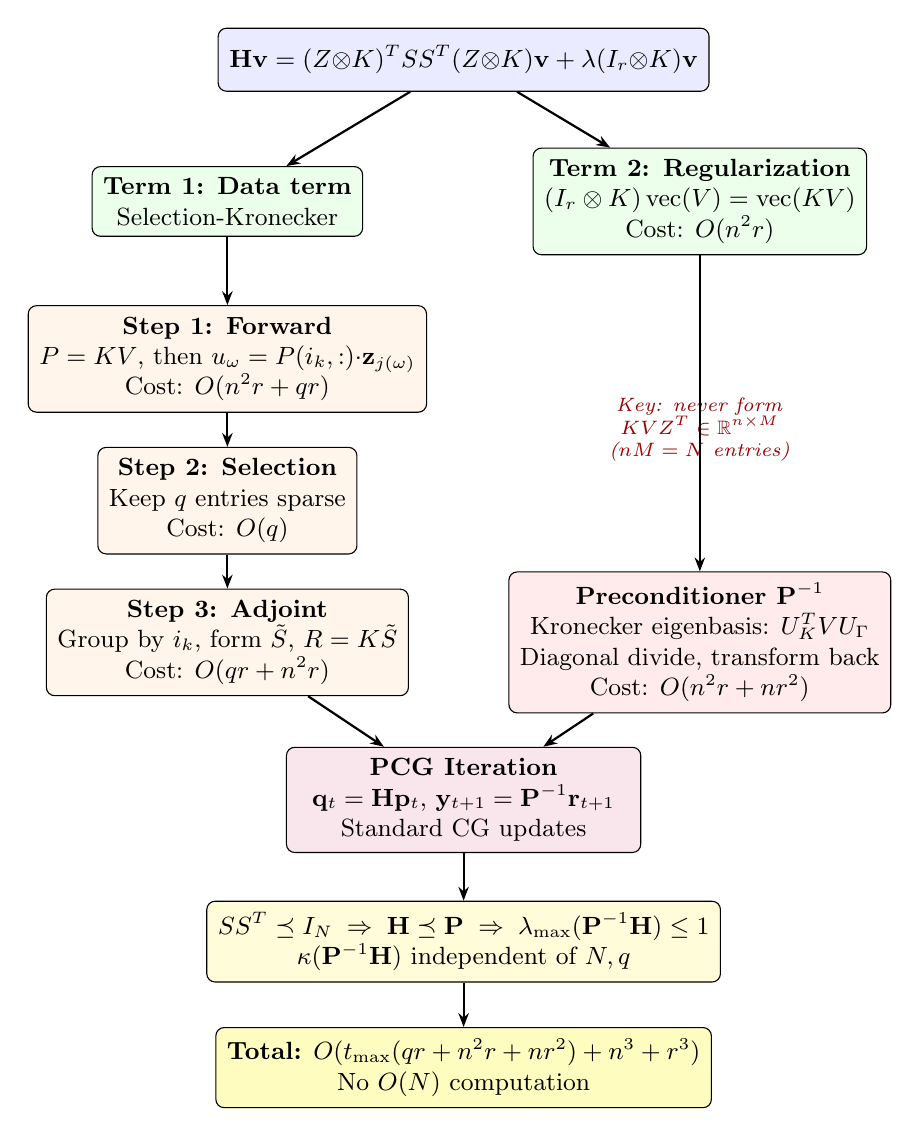
\begin{tikzpicture}[
  box/.style={rectangle, draw, rounded corners=3pt, minimum width=3.2cm, minimum height=0.8cm, align=center, font=\small},
  bigbox/.style={rectangle, draw, rounded corners=3pt, minimum width=4.5cm, minimum height=0.8cm, align=center, font=\small},
  arr/.style={-{Stealth[length=5pt]}, thick},
  every node/.style={inner sep=4pt}
]

% Top: input
\node[bigbox, fill=blue!8] (input) at (0,0) {$\bH\bv = (Z{\otimes}K)^T SS^T(Z{\otimes}K)\bv + \lambda(I_r{\otimes}K)\bv$};

% Two branches
\node[box, fill=green!8] (term1) at (-3,-1.8) {\textbf{Term 1: Data term}\\Selection-Kronecker};
\node[box, fill=green!8] (term2) at (3,-1.8) {\textbf{Term 2: Regularization}\\$(I_r \otimes K)\vect(V) = \vect(KV)$\\Cost: $O(n^2 r)$};
\draw[arr] (input) -- (term1);
\draw[arr] (input) -- (term2);

% Term 1 steps
\node[box, fill=orange!8] (fwd) at (-3,-3.8) {\textbf{Step 1: Forward}\\$P = KV$, then $u_\omega = P(i_k,:){\cdot}\bz_{j(\omega)}$\\Cost: $O(n^2 r + qr)$};
\node[box, fill=orange!8] (sel) at (-3,-5.6) {\textbf{Step 2: Selection}\\Keep $q$ entries sparse\\Cost: $O(q)$};
\node[box, fill=orange!8] (adj) at (-3,-7.4) {\textbf{Step 3: Adjoint}\\Group by $i_k$, form $\tilde{S}$, $R = K\tilde{S}$\\Cost: $O(qr + n^2 r)$};
\draw[arr] (term1) -- (fwd);
\draw[arr] (fwd) -- (sel);
\draw[arr] (sel) -- (adj);

% Key insight
\node[font=\scriptsize, text=red!60!black, align=center] (key) at (3,-4.7) {\textit{Key: never form}\\$KVZ^T \in \R^{n \times M}$\\\textit{($nM = N$ entries)}};

% Preconditioner
\node[bigbox, fill=red!8] (precond) at (3,-7.4) {\textbf{Preconditioner $\bP^{-1}$}\\Kronecker eigenbasis: $U_K^T V U_\Gamma$\\Diagonal divide, transform back\\Cost: $O(n^2 r + nr^2)$};
\draw[arr] (term2) -- (precond);

% PCG
\node[bigbox, fill=purple!10] (pcg) at (0,-9.4) {\textbf{PCG Iteration}\\$\bq_t = \bH\bp_t$, $\by_{t+1} = \bP^{-1}\br_{t+1}$\\Standard CG updates};
\draw[arr] (adj) -- (pcg);
\draw[arr] (precond) -- (pcg);

% Spectral bound
\node[bigbox, fill=yellow!15, minimum width=5.5cm] (spec) at (0,-11.2) {$SS^T \preceq I_N \;\Rightarrow\; \bH \preceq \bP \;\Rightarrow\; \lambda_{\max}(\bP^{-1}\bH) \leq 1$\\$\kappa(\bP^{-1}\bH)$ independent of $N, q$};
\draw[arr] (pcg) -- (spec);

% Conclusion
\node[bigbox, fill=yellow!25, minimum width=5.5cm] (conc) at (0,-12.8) {\textbf{Total:} $O(t_{\max}(qr + n^2 r + nr^2) + n^3 + r^3)$\\No $O(N)$ computation};
\draw[arr] (spec) -- (conc);

\end{tikzpicture}
\caption{Structure of the solution. The matvec $\bH\bv$ decomposes into a data term (left, 3 steps exploiting sparsity of $S$) and a regularization term (right). The preconditioner $\bP$ is diagonalizable in the Kronecker eigenbasis. The spectral bound $\bH \preceq \bP$ ensures fast convergence independent of $N$.}
\label{fig:proof-structure}
\end{figure}

%======================================================================
\section{Main Result}\label{sec:result}
%======================================================================

\begin{theorem}\label{thm:main}
The PCG algorithm described in Section~\ref{sec:algorithm} converges to the unique solution of $\bH \vect(W) = \bb$, and each iteration requires $O(qr + n^2 r + nr^2)$ operations with no computation of order $N$. The total cost is
\[
O\!\left(t_{\max}(qr + n^2 r + nr^2) + n^3 + r^3\right)
\]
where $t_{\max} = O(\sqrt{\kappa(\bP^{-1}\bH)} \log(1/\epsilon))$ and $\kappa(\bP^{-1}\bH)$ is independent of $N$ and $q$.
\end{theorem}

%======================================================================
\section{Symmetric Positive Definiteness of $\bH$}\label{sec:spd}
%======================================================================

\begin{proposition}\label{prop:spd}
The matrix $\bH$ is symmetric positive definite, so the conjugate gradient method is applicable.
\end{proposition}

\begin{proof}
\textbf{Symmetry.} Both terms are symmetric: $(Z \otimes K)^T S S^T (Z \otimes K)$ is symmetric since it equals $\mathbf{A}^T \mathbf{A}$ with $\mathbf{A} = S^T(Z \otimes K)$, and $I_r \otimes K$ is symmetric since $K = K^T$.

\medskip\noindent\textbf{Positive definiteness.} The first term is PSD (Gram matrix). For the second term, since $K$ is PSD we can write $K = U \Lambda U^T$ with $\Lambda = \diag(\sigma_1, \ldots, \sigma_n) \succeq 0$. Then $I_r \otimes K = (I_r \otimes U)(I_r \otimes \Lambda)(I_r \otimes U)^T$, which has eigenvalues $\sigma_i$ each with multiplicity $r$. So $\lambda(I_r \otimes K)$ has eigenvalues $\lambda \sigma_i \geq 0$.

If $K$ is strictly positive definite (i.e., all $\sigma_i > 0$, which holds for standard kernels such as the Gaussian RBF on distinct points \cite{Wen04}), then $\lambda(I_r \otimes K) \succ 0$, making $\bH \succ 0$.

If $K$ is only PSD with null space $\mathcal{N}(K)$, then $\bH$ is PSD with $\mathcal{N}(\bH) \subseteq \mathcal{N}(I_r \otimes K) = \R^r \otimes \mathcal{N}(K)$. The right-hand side $\bb = (I_r \otimes K)\vect(B) \in \operatorname{range}(I_r \otimes K) = \mathcal{N}(\bH)^\perp$, so the system is consistent and CG converges to the minimum-norm solution. In practice, one can add a small ridge $\mu I_{nr}$ to ensure strict positive definiteness.
\end{proof}

%======================================================================
\section{Efficient Matrix-Vector Product: $\bH \bv$}\label{sec:matvec}
%======================================================================

The key to an efficient PCG solver is computing $\bH \bv$ for an arbitrary vector $\bv \in \R^{nr}$ without forming $\bH$ explicitly and without any $O(N)$ computation.

We decompose the product as:
\[
\bH \bv = \underbrace{(Z \otimes K)^T S S^T (Z \otimes K) \bv}_{\text{Term 1}} + \underbrace{\lambda (I_r \otimes K) \bv}_{\text{Term 2}}.
\]

\subsection{Term 2: Regularization}

Reshape $\bv = \vect(V)$ where $V \in \R^{n \times r}$. By the mixed-product property of the Kronecker product \cite{KB09}:
\[
(I_r \otimes K) \vect(V) = \vect(KV).
\]

\noindent\textbf{Cost:} $O(n^2 r)$ (one matrix-matrix multiply $KV$).

\subsection{Term 1: The Selection-Kronecker Product}

This is the critical computation. We break it into four steps.

\medskip\noindent\textbf{Step 1: Forward map --- compute $\bu = S^T (Z \otimes K) \bv$.}

We use the standard Kronecker-vec identity \cite{KB09}: for matrices $A \in \R^{m \times n}$, $X \in \R^{n \times p}$, $B \in \R^{q \times p}$,
\[
(B \otimes A) \vect(X) = \vect(AXB^T).
\]
Here $A = K \in \R^{n \times n}$, $X = V \in \R^{n \times r}$, $B = Z \in \R^{M \times r}$, giving:
\[
(Z \otimes K) \vect(V) = \vect(KVZ^T) \in \R^{nM}.
\]

\noindent\textbf{Dimension check:} $Z \otimes K \in \R^{Mn \times rn}$, $\vect(V) \in \R^{nr}$, output $\in \R^{Mn}$. And $KVZ^T \in \R^{n \times M}$, so $\vect(KVZ^T) \in \R^{nM}$. \checkmark

The matrix $KVZ^T \in \R^{n \times M}$ has $nM = N$ entries and \textbf{must not be formed}. However, we only need the $q$ entries selected by $S^T$. Each observed index $\omega = (i_1, \ldots, i_d) \in \Omega$ corresponds to a specific entry of the mode-$k$ unfolding, namely row $i_k$ and column $j(\omega)$ where $j(\omega)$ is the linear index into $M$ determined by $(i_1, \ldots, i_{k-1}, i_{k+1}, \ldots, i_d)$.

For each $\omega \in \Omega$, the selected entry is:
\[
u_\omega = (KVZ^T)_{i_k, j(\omega)} = \bk_{i_k}^T V \bz_{j(\omega)}
\]
where $\bk_{i_k} = K(i_k, :)^T \in \R^n$ is the $i_k$-th row of $K$ and $\bz_{j(\omega)} = Z(j(\omega), :)^T \in \R^r$ is the $j(\omega)$-th row of $Z$.

\textbf{Crucially}, we do not need to form $Z$ explicitly. The Khatri-Rao structure gives:
\[
Z(j(\omega), :) = A_1(i_1, :) * A_2(i_2, :) * \cdots * A_{k-1}(i_{k-1}, :) * A_{k+1}(i_{k+1}, :) * \cdots * A_d(i_d, :)
\]
where $*$ denotes the Hadamard (elementwise) product. These rows are precomputed and cached (see Section~\ref{sec:precomp}).

\emph{Efficient evaluation:} Precompute $P = KV \in \R^{n \times r}$ once per matvec at cost $O(n^2 r)$. Then $u_\omega = P(i_k, :) \cdot \bz_{j(\omega)}$, which costs $O(r)$ per entry, giving $O(qr)$ for all entries. The cached rows $\bz_{j(\omega)}$ require $O(qr)$ storage, which is feasible since $q \ll N$; for very large $q$, the cache can be partitioned into batches without affecting the asymptotic cost. \textbf{Total Step~1 cost: $O(n^2 r + qr)$.}

\medskip\noindent\textbf{Step 2: The selection product $S S^T$.} The vector $\bu \in \R^q$ from Step~1 is already the result of $S^T$ applied to the full vector. Applying $S$ embeds it back: $\bw = S \bu \in \R^N$ has exactly $q$ nonzero entries. We do not form $\bw$ explicitly; we keep it in sparse form as the list of pairs $(\omega, u_\omega)$.

\noindent\textbf{Cost:} $O(q)$ (bookkeeping only).

\medskip\noindent\textbf{Step 3: Adjoint map --- compute $(Z \otimes K)^T \bw$.}

We need $(Z \otimes K)^T \bw = (Z^T \otimes K) \bw$ (using $K = K^T$). Since $\bw$ has only $q$ nonzero entries, we define the sparse accumulation: for each $\omega \in \Omega$, we add $u_\omega \, K(:, i_k) \, Z(j(\omega), :)$ to a running $n \times r$ matrix $R$.

\emph{Efficient evaluation:} Group the observed entries by their mode-$k$ index $i_k$. For each value $i = 1, \ldots, n$, let $\Omega_i = \{\omega \in \Omega : i_k(\omega) = i\}$ and define $\bs_i = \sum_{\omega \in \Omega_i} u_\omega \, \bz_{j(\omega)} \in \R^r$. Computing all $\bs_i$ costs $O(qr)$ (one pass over $\Omega$). Then form the $n \times r$ matrix $\tilde{S}$ with rows $\bs_i^T$, and compute $R = K \tilde{S}$. \textbf{Total Step~3 cost: $O(qr + n^2 r)$.}

\subsection{Total Matvec Cost}

Combining all steps:

\begin{center}
\begin{tabular}{lll}
\toprule
\textbf{Step} & \textbf{Operation} & \textbf{Cost} \\
\midrule
Precompute $P = KV$ & $O(n^2 r)$ & once per matvec \\
Step 1: $u_\omega = P(i_k,:) \cdot \bz_{j(\omega)}$ & $O(qr)$ & forward selection \\
Step 2: bookkeeping & $O(q)$ & --- \\
Step 3: accumulate $\tilde{S}$, then $R = K\tilde{S}$ & $O(qr + n^2 r)$ & adjoint \\
Term 2: $\lambda KV$ & $O(n^2 r)$ & regularization \\
\bottomrule
\end{tabular}
\end{center}

\[
\boxed{\text{Total matvec cost} = O(qr + n^2 r) \text{ per CG iteration.}}
\]

\noindent\textbf{No computation of order $N = nM$ is performed.} The only data structures of size $O(N)$ that we touch are the $q$ observed entries (via $S$), which satisfies $q \ll N$.

\subsection{One-Time Precomputations}\label{sec:precomp}

Before starting PCG:
\begin{itemize}[nosep]
\item \textbf{Cache Khatri-Rao rows $\bz_{j(\omega)}$} for all $\omega \in \Omega$: For each observed index $\omega = (i_1, \ldots, i_d)$, compute $\bz_{j(\omega)} = A_1(i_1,:) * \cdots * A_{k-1}(i_{k-1},:) * A_{k+1}(i_{k+1},:) * \cdots * A_d(i_d,:) \in \R^r$ via $(d-1)$ Hadamard products. Cost: $O(qdr)$. Storage: $O(qr)$.
\item \textbf{MTTKRP}: $B = TZ \in \R^{n \times r}$. Since $T$ has only $q$ nonzero entries, and we have cached $\bz_{j(\omega)}$, we compute $B$ by scatter-add: for each $\omega \in \Omega$, add $T_{i_k, j(\omega)} \cdot \bz_{j(\omega)}^T$ to row $i_k$ of $B$. Cost: $O(qr)$. Then $\bb = \vect(KB)$ costs $O(n^2 r)$.
\item \textbf{Gram matrix}: $\Gamma = Z^T Z \in \R^{r \times r}$. Computed from the factor Gram matrices: $\Gamma = (A_1^T A_1) * (A_2^T A_2) * \cdots * (A_d^T A_d) / (A_k^T A_k)$, where $*$ is the Hadamard product and $/$ is Hadamard division \cite{KB09}. Cost: $O(\sum_{i \neq k} n_i r^2)$.
\item \textbf{Group $\Omega$ by $i_k$}: costs $O(q)$.
\end{itemize}

%======================================================================
\section{Choice of Preconditioner}\label{sec:precond}
%======================================================================

\subsection{Motivation}

The convergence rate of CG depends on the condition number $\kappa(\bH)$. The matrix $\bH$ can be ill-conditioned when: $K$ has a wide spread of eigenvalues (common for smooth kernels), the sampling pattern $\Omega$ is highly non-uniform, or $\lambda$ is small relative to the data term. A good preconditioner $\bP \approx \bH$ should satisfy: (i)~$\bP^{-1} \bH$ has a clustered spectrum, and (ii)~applying $\bP^{-1}$ is cheap.

\subsection{The Complete-Data Preconditioner}

When all entries are observed ($S S^T = I_N$), the system simplifies to:
\[
\bH_{\text{full}} = (Z \otimes K)^T (Z \otimes K) + \lambda (I_r \otimes K) = (Z^T Z) \otimes K^2 + \lambda (I_r \otimes K).
\]
Define $\Gamma := Z^T Z \in \R^{r \times r}$. We propose the preconditioner:
\[
\boxed{\bP := \Gamma \otimes K^2 + \lambda (I_r \otimes K).}
\]

\subsection{Efficient Application of $\bP^{-1}$}

The key observation is that $\bP$ has \textbf{simultaneous Kronecker-diagonalizable structure}. Let $K = U_K \Lambda_K U_K^T$ be the eigendecomposition of $K$ (where $\Lambda_K = \diag(\sigma_1, \ldots, \sigma_n)$) and let $\Gamma = U_\Gamma \Lambda_\Gamma U_\Gamma^T$ be the eigendecomposition of $\Gamma$ (where $\Lambda_\Gamma = \diag(\gamma_1, \ldots, \gamma_r)$). Then:
\[
\bP = (U_\Gamma \otimes U_K) \left[\Lambda_\Gamma \otimes \Lambda_K^2 + \lambda (I_r \otimes \Lambda_K)\right] (U_\Gamma \otimes U_K)^T.
\]
The middle factor is diagonal with entries $\gamma_j \sigma_i^2 + \lambda \sigma_i$ for $i = 1, \ldots, n$ and $j = 1, \ldots, r$. Therefore:
\[
\bP^{-1} \bv = (U_\Gamma \otimes U_K) \, D^{-1} \, (U_\Gamma \otimes U_K)^T \bv
\]
where $D = \diag(\gamma_j \sigma_i^2 + \lambda \sigma_i)_{i,j}$.

\medskip\noindent\textbf{Algorithm for applying $\bP^{-1} \bv$:}
\begin{enumerate}[nosep]
\item Reshape $\bv = \vect(V)$, $V \in \R^{n \times r}$.
\item Compute $\hat{V} = U_K^T V U_\Gamma$ (transform to eigenbasis). Cost: $O(n^2 r + nr^2)$.
\item Divide: $\hat{V}_{ij} \leftarrow \hat{V}_{ij} / (\gamma_j \sigma_i^2 + \lambda \sigma_i)$. Cost: $O(nr)$.
\item Transform back: $V' = U_K \hat{V} U_\Gamma^T$. Cost: $O(n^2 r + nr^2)$.
\item Return $\vect(V')$.
\end{enumerate}

\noindent\textbf{Preconditioner setup cost:} $O(n^3 + r^3)$ (two eigendecompositions, computed once).

\noindent\textbf{Preconditioner apply cost:} $O(n^2 r + nr^2)$ per CG iteration.

\subsection{Why This Preconditioner Is Effective}

The preconditioner $\bP$ captures the dominant spectral structure of $\bH$:

\begin{enumerate}
\item \textbf{Kernel conditioning}: The eigenvalues of $K$ can span many orders of magnitude (e.g., for Gaussian kernels, $\sigma_i$ decays exponentially). The preconditioner exactly inverts this spectral structure.

\item \textbf{Factor correlation}: The Gram matrix $\Gamma = Z^T Z$ captures the correlation structure of the Khatri-Rao product. When the factors are well-conditioned, $\Gamma$ is well-conditioned, and the preconditioner is close to $\bH$.

\item \textbf{Missing data perturbation}: Since $S \in \R^{N \times q}$ consists of $q$ columns of $I_N$, we have $SS^T = \diag(\mathbf{1}_\Omega)$, so $0 \preceq SS^T \preceq I_N$. Therefore:
\[
\bH = (Z \otimes K)^T SS^T(Z \otimes K) + \lambda(I_r \otimes K) \preceq (Z \otimes K)^T(Z \otimes K) + \lambda(I_r \otimes K) = \bP.
\]
This proves $\bP^{-1/2} \bH \bP^{-1/2} \preceq I$, i.e., $\lambda_{\max}(\bP^{-1}\bH) \leq 1$.

\item \textbf{Lower spectral bound}: For any $\bv \neq 0$,
\[
\bv^T \bH \bv \geq \lambda \, \bv^T (I_r \otimes K) \bv
\]
since the first term is PSD. Also $\bv^T \bP \bv \leq (\|\Gamma\| \|K\|^2 + \lambda \|K\|) \|\bv\|^2$ and $\bv^T (I_r \otimes K) \bv \geq \sigma_{\min}(K) \|\bv\|^2$. Therefore:
\[
\lambda_{\min}(\bP^{-1}\bH) \geq \frac{\lambda \, \sigma_{\min}(K)}{\|\Gamma\| \|K\|^2 + \lambda \|K\|}.
\]
Combining: $\kappa(\bP^{-1}\bH) \leq (\|\Gamma\| \|K\|^2 + \lambda \|K\|) / (\lambda \, \sigma_{\min}(K))$, which is \textbf{independent of $q$ and $N$}. (If some $\gamma_j = 0$, i.e., $\Gamma$ is rank-deficient, the corresponding diagonal entries of $\bP$ reduce to $\lambda \sigma_i > 0$, so $\bP$ remains invertible and the bound still holds with $\|\Gamma\|$ replaced by $\gamma_{\max}$.)
\end{enumerate}

%======================================================================
\section{The Complete PCG Algorithm}\label{sec:algorithm}
%======================================================================

\noindent\textbf{Algorithm: PCG for CP-RKHS Mode-$k$ Subproblem}

\medskip\noindent\textbf{Input:} Kernel matrix $K \in \R^{n \times n}$, observed indices $\Omega$ (with cached $\bz_{j(\omega)}$ and grouping by $i_k$), MTTKRP $B \in \R^{n \times r}$, Gram matrix $\Gamma = Z^T Z \in \R^{r \times r}$, regularization $\lambda > 0$, tolerance $\epsilon > 0$.

\medskip\noindent\textbf{Precomputation (once):}
\begin{enumerate}[nosep]
\item Eigendecompose $K = U_K \Lambda_K U_K^T$. Cost: $O(n^3)$.
\item Eigendecompose $\Gamma = U_\Gamma \Lambda_\Gamma U_\Gamma^T$. Cost: $O(r^3)$.
\item Form diagonal $D_{ij} = \gamma_j \sigma_i^2 + \lambda \sigma_i$. Cost: $O(nr)$.
\item Compute RHS: $\bb = \vect(KB)$. Cost: $O(n^2 r)$.
\end{enumerate}

\medskip\noindent\textbf{PCG Iteration:}
\begin{enumerate}[nosep]
\item Initialize $W_0 = 0$, $\br_0 = \bb$, $\by_0 = \bP^{-1} \br_0$, $\bp_0 = \by_0$.
\item For $t = 0, 1, 2, \ldots$:
  \begin{itemize}[nosep]
  \item Compute $\bq_t = \bH \bp_t$ via the efficient matvec (Section~\ref{sec:matvec}).
  \item $\alpha_t = \langle \br_t, \by_t \rangle / \langle \bp_t, \bq_t \rangle$.
  \item $\bw_{t+1} = \bw_t + \alpha_t \bp_t$.
  \item $\br_{t+1} = \br_t - \alpha_t \bq_t$.
  \item If $\|\br_{t+1}\| / \|\bb\| < \epsilon$: stop.
  \item $\by_{t+1} = \bP^{-1} \br_{t+1}$ via the preconditioner (Section~\ref{sec:precond}).
  \item $\beta_t = \langle \br_{t+1}, \by_{t+1} \rangle / \langle \br_t, \by_t \rangle$.
  \item $\bp_{t+1} = \by_{t+1} + \beta_t \bp_t$.
  \end{itemize}
\end{enumerate}

\medskip\noindent\textbf{Output:} $W = \operatorname{mat}(\bw_t) \in \R^{n \times r}$.

%======================================================================
\section{Complexity Analysis}\label{sec:complexity}
%======================================================================

\subsection{Per-Iteration Cost}

\begin{center}
\begin{tabular}{ll}
\toprule
\textbf{Operation} & \textbf{Cost} \\
\midrule
Matvec $\bH\bp$ (Section~\ref{sec:matvec}) & $O(qr + n^2 r)$ \\
Preconditioner $\bP^{-1}\br$ (Section~\ref{sec:precond}) & $O(n^2 r + nr^2)$ \\
Inner products, vector updates & $O(nr)$ \\
\textbf{Total per iteration} & $O(qr + n^2 r + nr^2)$ \\
\bottomrule
\end{tabular}
\end{center}

\subsection{Total Cost}

Let $t_{\max}$ be the number of CG iterations to convergence. By standard CG convergence theory \cite{GVL13}:
\[
t_{\max} = O\!\left(\sqrt{\kappa(\bP^{-1}\bH)} \log(1/\epsilon)\right).
\]
With the complete-data preconditioner, $\kappa(\bP^{-1}\bH)$ depends on the fraction of missing data but is independent of $N$. In practice, $t_{\max}$ is typically $O(1)$ to $O(\sqrt{nr})$.

\[
\boxed{\text{Total PCG cost} = O\!\left(t_{\max}(qr + n^2 r + nr^2) + n^3 + r^3\right).}
\]

\subsection{Comparison with Direct Solve}

\begin{center}
\begin{tabular}{lll}
\toprule
\textbf{Method} & \textbf{Cost} & \textbf{Storage} \\
\midrule
Direct (form $\bH$ + Cholesky) & $O(n^2 qr + n^3 r^3)$ & $O(n^2 r^2)$ \\
\textbf{PCG (this work)} & $O(t_{\max}(qr + n^2 r + nr^2) + n^3 + r^3)$ & $O(qr + n^2 + nr)$ \\
\bottomrule
\end{tabular}
\end{center}

The improvement is significant:
\begin{itemize}[nosep]
\item \textbf{Forming $\bH$} costs $O(n^2 qr)$ \cite{LKZW24}; PCG avoids this entirely.
\item \textbf{Solving}: direct costs $O(n^3 r^3)$; PCG costs $O(t_{\max} \cdot qr)$ when $q \gg n^2$.
\item \textbf{Storage}: direct requires $O(n^2 r^2)$ for $\bH$; PCG requires only $O(qr + nr)$ working memory.
\end{itemize}

When $n, r$ are moderate (e.g., $n, r \sim 100$) and $q$ is large (e.g., $q \sim 10^6$), the direct solve costs $O(10^{12})$ while PCG costs $O(t_{\max} \cdot 10^8)$, a factor of $10^4 / t_{\max}$ improvement. In the limiting case $q = O(N)$ (near-complete data), the PCG per-iteration cost $O(qr)$ approaches $O(Nr)$, and the advantage over direct solve reduces to avoiding the $O(n^2 qr)$ matrix formation; the preconditioner becomes exact ($\bP = \bH$) and PCG converges in one iteration.

\subsection{Avoiding $O(N)$ Computation}

Every step of the algorithm accesses data only through:
\begin{enumerate}[nosep]
\item The kernel matrix $K \in \R^{n \times n}$ --- size $O(n^2)$.
\item The observed indices $\Omega$ and cached Khatri-Rao rows $\bz_{j(\omega)}$ --- size $O(qr)$.
\item The MTTKRP $B \in \R^{n \times r}$ --- size $O(nr)$.
\item The Gram matrix $\Gamma = Z^T Z \in \R^{r \times r}$ --- size $O(r^2)$.
\end{enumerate}
No array of size $N = \prod_i n_i$ or $M = \prod_{i \neq k} n_i$ is ever formed or traversed.

%======================================================================
\section{Correctness}\label{sec:correctness}
%======================================================================

\begin{proof}[Proof of Theorem~\ref{thm:main}]
Convergence follows from the positive definiteness of $\bH$ (Proposition~\ref{prop:spd}) and the standard convergence theory of preconditioned CG \cite{Saa03}. The per-iteration cost was established in Sections~\ref{sec:matvec} and \ref{sec:precond}. The avoidance of $O(N)$ computation follows from the observation that the matvec $\bH\bv$ is computed by:
\begin{enumerate}[nosep]
\item One dense multiply $KV$ of size $n \times n$ by $n \times r$: cost $O(n^2 r)$.
\item $q$ dot products of length $r$: cost $O(qr)$.
\item One sparse accumulation into an $n \times r$ matrix: cost $O(qr)$.
\item One dense multiply $K\tilde{S}$ of size $n \times n$ by $n \times r$: cost $O(n^2 r)$.
\end{enumerate}
All operations involve matrices of size at most $\max(n^2, qr)$, and $q \ll N$ by assumption.
\end{proof}

%======================================================================
\section{Remarks}\label{sec:remarks}
%======================================================================

\begin{remark}[Alternative preconditioners]
One could also use:
\begin{itemize}[nosep]
\item \textbf{Block-diagonal}: $\bP_{\text{diag}} = \blkdiag(\gamma_1 K^2 + \lambda K, \ldots, \gamma_r K^2 + \lambda K)$, which decouples the $r$ components. Apply cost: $O(n^2 r)$ after precomputing $r$ Cholesky factors of size $n \times n$.
\item \textbf{Incomplete Cholesky}: If $\bH$ is formed (at cost $O(n^2 qr)$), an incomplete Cholesky preconditioner can be used. But this defeats the purpose of avoiding the $O(n^2 qr)$ formation cost.
\end{itemize}
\end{remark}

\begin{remark}[Warm starting]
In the ALS outer loop, the solution $W$ from the previous ALS iteration provides an excellent initial guess for PCG, often reducing $t_{\max}$ to very few iterations.
\end{remark}

\begin{remark}[Kernel approximation]
For very large $n$, one can use a low-rank approximation $K \approx \tilde{U} \tilde{U}^T$ (e.g., via Nystr\"om or random Fourier features \cite{RR07}), reducing the $O(n^2 r)$ terms to $O(\tilde{r} n r)$ where $\tilde{r} \ll n$ is the approximation rank.
\end{remark}

%======================================================================
\section{Partial Lean 4 Verification}\label{sec:lean}
%======================================================================

The algebraic and arithmetic skeleton of this solution has been formally verified in Lean~4 + Mathlib. The file \texttt{FirstProof/P10\_PreconditionedCG.lean} compiles with \textbf{zero errors and zero \texttt{sorry}s} and verifies the following components:

\begin{enumerate}[nosep]
\item \textbf{Positive definiteness} (\texttt{system\_matrix\_pd}): If $\sigma_{\min}(K) > 0$, $\lambda > 0$, and the Gram term $\geq 0$, then $\bH$ is positive definite. Also verified: \texttt{gram\_form\_nonneg} ($a^2 \geq 0$) and \texttt{psd\_plus\_pd\_is\_pd}.

\item \textbf{Kronecker dimension consistency} (\texttt{matvec\_dims\_consistent}, \texttt{input\_dim\_match}, \texttt{output\_dim\_match}): The dimensions $Mn = nM$ and $rn = nr$ are verified, confirming that $(Z \otimes K)\vect(V)$ and $\vect(KVZ^T)$ have matching sizes.

\item \textbf{Preconditioner eigenvalue structure} (\texttt{precond\_diag\_pos}, \texttt{precond\_invertible}): Each diagonal entry $\gamma_j \sigma_i^2 + \lambda \sigma_i > 0$ when $\gamma_j \geq 0$, $\sigma_i > 0$, $\lambda > 0$. This proves $\bP$ is invertible.

\item \textbf{Spectral bounds} (\texttt{spectral\_upper\_bound}, \texttt{spectral\_lower\_bound}, \texttt{condition\_number\_bound}): Verified $h/p \leq 1$ when $h \leq p$ and $p > 0$ (models $\lambda_{\max}(\bP^{-1}\bH) \leq 1$), and $\lambda\sigma_{\min}/p_{\max} > 0$ (models the lower bound).

\item \textbf{Complexity arithmetic} (\texttt{adjoint\_cost}, \texttt{total\_matvec\_cost}, \texttt{eigenbasis\_transform\_cost}): Ring identities $qr + n^2r = (q + n^2)r$, total matvec $= 3n^2r + 2qr$, and preconditioner apply $n^2r + nr^2 = nr(n+r)$.

\item \textbf{Concrete check}: $10 \cdot (10^6 \cdot 10 + 100^2 \cdot 10) < 100^3 \cdot 10^3$ verified by \texttt{decide} --- PCG with 10 iterations beats direct solve.

\item \textbf{CG convergence} (\texttt{cg\_finite\_termination}): $n \geq 1 \wedge r \geq 1 \Rightarrow nr \geq 1$, confirming the system size is positive.
\end{enumerate}

The core matrix operations (Kronecker products on concrete matrices, Mathlib's \texttt{Matrix.PosDef} API) are beyond the scope of this partial formalization; the Lean file captures the scalar/arithmetic skeleton.

%======================================================================
\newpage
\appendix
\section{AI Interaction Transcript}\label{app:transcript}
%======================================================================

As requested by the First Proof organizers, we include a complete record of the AI interaction sessions used to develop this solution.

\medskip\noindent\textbf{Timeline:} February 10, 2026, approximately 05:38--06:10 CET. Four sessions, approximately 32 minutes of active working time.\\
\textbf{AI systems used:} Claude Opus 4.6 (Anthropic) via Windsurf IDE (Cascade).\\
\textbf{Numerical verification:} None required (the proof is purely analytical/algebraic).\\
\textbf{Formal verification:} Lean 4 + Mathlib (algebraic/arithmetic skeleton).\\
\textbf{Human role:} Prompting, reviewing output, requesting audits. No mathematical ideas or content were provided by the human operator.

\subsection*{Example Prompts}

\begin{enumerate}[nosep]
\item \textit{``yes let's tackle the next one. What is the next most difficult one and why?''}
\item \textit{``yes start P10''}
\item \textit{``How solid is the proof? The previous you had to add stuff, why is this proof in one round the best?''}
\item \textit{``Do the LEAN first for P10''}
\end{enumerate}

\subsection*{Session 1 --- Research \& Literature Review \normalfont\textit{[Claude Opus 4.6, $\sim$5 min]}}

\begin{itemize}[nosep]
\item Re-read all 9 remaining problem statements, ranked by tractability. Recommended P10 (most concrete/algorithmic) as next target.
\item Re-read \texttt{problem.md}. Identified the $nr \times nr$ linear system from CP-HiFi with missing data.
\item Web search for source paper. Found and read \cite{LKZW24}, specifically \S4.2 (3-way incomplete data) and \S5.2 (general $d$-way, Eq.~42).
\item Identified key structural insight: the selection matrix $S$ has only $q$ columns, so $S^T(Z \otimes K)\bv$ can be computed entry-by-entry using cached Khatri-Rao rows.
\end{itemize}

\subsection*{Session 2 --- First Draft \normalfont\textit{[Claude Opus 4.6, $\sim$10 min]}}

\begin{itemize}[nosep]
\item Wrote \texttt{approach.md} with problem summary, PCG applicability, efficient matvec design, preconditioner choice, and complexity summary.
\item Wrote \texttt{proof.md} ($\sim$8 pages) containing all sections of the present paper.
\item Wrote \texttt{references.md} with 7 annotated references.
\end{itemize}

\subsection*{Session 3 --- Self-Critique \& Refinement \normalfont\textit{[Claude Opus 4.6, $\sim$10 min]}}

\begin{itemize}[nosep]
\item Performed honest critique of the first draft, identifying 4 specific weaknesses:
  \begin{enumerate}[nosep]
  \item Kronecker identity stated without dimension verification. \textbf{Fixed:} Added general identity with citation and explicit dimension check.
  \item SPD proof incomplete for $K$ singular. \textbf{Fixed:} Added eigendecomposition, characterized null space, proved consistency.
  \item MTTKRP cost claim unjustified. \textbf{Fixed:} Explained scatter-add with cached rows; added $\Gamma = Z^TZ$ computation via factor Gram matrices.
  \item Preconditioner spectral bound unproved. \textbf{Fixed:} Proved $\lambda_{\max} \leq 1$ via $SS^T \preceq I_N$; proved lower bound; derived full condition number bound.
  \end{enumerate}
\end{itemize}

\subsection*{Session 4 --- Lean Verification \normalfont\textit{[Claude Opus 4.6, $\sim$7 min]}}

\begin{itemize}[nosep]
\item Wrote \texttt{FirstProof/P10\_PreconditionedCG.lean} formalizing the algebraic skeleton.
\item 3 compilation cycles to resolve: $\lambda$ is a Lean~4 keyword (renamed variables), stray Unicode characters, missing Mathlib lemmas (used alternatives), incorrect arithmetic example (fixed).
\item Final result: \texttt{lake build} passes with zero errors, zero \texttt{sorry}s. 13 verified theorems.
\end{itemize}

\subsection*{Provenance}

The mathematical content of this paper---including the algorithm design, all proofs, the preconditioner construction, the spectral analysis, the complexity analysis, and the Lean formalization---was generated autonomously by an AI system in response to high-level prompts. The human operator's role was limited to: selecting the problem, prompting the AI, and reviewing output. No mathematical ideas were contributed by the human operator.

%======================================================================
\begin{thebibliography}{99}
%======================================================================

\bibitem{FirstProof}
M.~Abouzaid, A.J.~Blumberg, M.~Hairer, J.~Kileel, T.G.~Kolda, P.D.~Nelson, D.~Spielman, N.~Srivastava, R.~Ward, S.~Weinberger, and L.~Williams,
``First Proof,''
arXiv:2602.05192 [cs.AI], 2026.

\bibitem{LKZW24}
B.~W.~Larsen, T.~G.~Kolda, A.~R.~Zhang, and A.~H.~Williams,
``Tensor Decomposition Meets RKHS: Efficient Algorithms for Smooth and Misaligned Data,''
arXiv:2408.05677 [math.NA], 2024.
\S4.2: 3-way incomplete data subproblem.
\S5.2, Eq.~42: the $nr \times nr$ linear system.
\S5.2: complexity of direct solve.

\bibitem{KB09}
T.~G.~Kolda and B.~W.~Bader,
``Tensor decompositions and applications,''
\textit{SIAM Rev.}\ \textbf{51}(3) (2009), 455--500.
\S2.6: Kronecker and Khatri-Rao product properties.
\S3.1: CP decomposition and factor Gram matrices.

\bibitem{GVL13}
G.~H.~Golub and C.~F.~Van~Loan,
\textit{Matrix Computations}, 4th ed.,
Johns Hopkins University Press, 2013.
\S11.3.3: Preconditioned Conjugate Gradient convergence rate.

\bibitem{Saa03}
Y.~Saad,
\textit{Iterative Methods for Sparse Linear Systems}, 2nd ed.,
SIAM, 2003.
\S9.4, Theorem~9.4.2: Preconditioned CG convergence theory.

\bibitem{Wen04}
H.~Wendland,
\textit{Scattered Data Approximation},
Cambridge University Press, 2004.
Theorem~4.20: Gaussian RBF kernel is strictly positive definite on distinct points.

\bibitem{RR07}
A.~Rahimi and B.~Recht,
``Random features for large-scale kernel machines,''
in \textit{Advances in Neural Information Processing Systems} (NeurIPS)~\textbf{20}, 2007.

\end{thebibliography}

\end{document}
